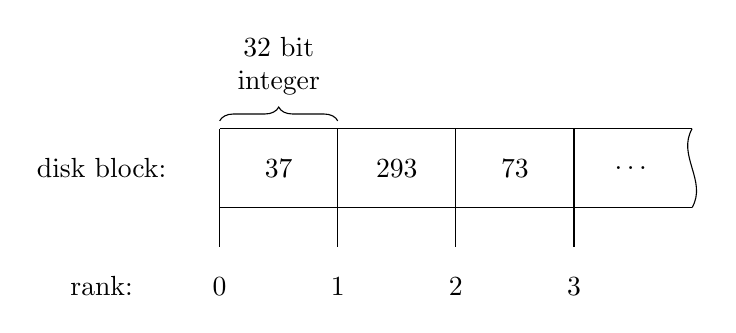
\begin{tikzpicture}[node distance={15mm}, main/.style = {draw, circle}]

    \draw (0,0) -- (6,0);
    \draw (0,1) -- (6,1);
    \draw (0,-0.5) -- (0,1);
    \draw (1.5,-0.5) -- (1.5,1);
    \draw (3,-0.5) -- (3,1);
    \draw (4.5,-0.5) -- (4.5,1);
    \draw[out=60, in=-120] (6,0) to (6,1);

    \node at (0.75, 0.5) {37};
    \node at (2.25, 0.5) {293};
    \node at (3.75, 0.5) {73};
    \node at (5.25, 0.5) {…};

    \node at (-1.5, 0.5) {disk block:};
    \node at (-1.5, -1) {rank:};
    \node at (0, -1) {0};
    \node at (1.5, -1) {1};
    \node at (3, -1) {2};
    \node at (4.5, -1) {3};

    \draw [decorate,decoration = {brace, amplitude=5pt}] (0,1.1) --  (1.5,1.1);
    \node[ align=center] at (0.75, 1.8) {32 bit  \\ integer};

\end{tikzpicture}